%!TEX root = TIWSNE_Mini_project_main.tex
\section{Wireless transmission}
This project focuses on image compression and energy comparison, but when transmitting data wireless, one must always consider reliability.
Transmission over a wireless channel, is in nature unreliable due to fading, interference, loss of bit synchronization, just to mention some causes.

There are four major criteria associated with a reliable transmission:
\begin{itemize}
\item No lost packages.
\item Error-free packets.
\item Packets must be in-sequence.
\item No duplicate packets.
\end{itemize}
To achieve all these criteria there is two approaches:
\begin{itemize}
\item Automatic Repeat-reQuest (ARQ), which is a reactive approach.
\item Forward Error Control, which is a proactive approach. 
\end{itemize}

The FEC adds redundancy bits to the sent packet and thus decreases the packet error rate.
The encoding and decoding requires implementing a block code, such as the Reed-Soloman code.
This project does not focus on FEC or block codes, so this approach is discarded.
Further it is assumed that the wireless channel is good, and the transmitting distance is very small, so the increased packet error rate might be negligible.
The FEC approach alone does not guarantee an error free transmission, it only improves the error rate.

The three most common ARQ methods can be seen in Figure \ref{fig:ARQ}. The Stop-and-Wait method is the simplest, slowest and most power consuming. The receiver sends a positive acknowledgment for every packet, and the transmitter only transmits one packet at a time. If an acknowledgment is not received within a certain timeout limit, the sender retransmits the last packet.

\begin{figure}
\centering
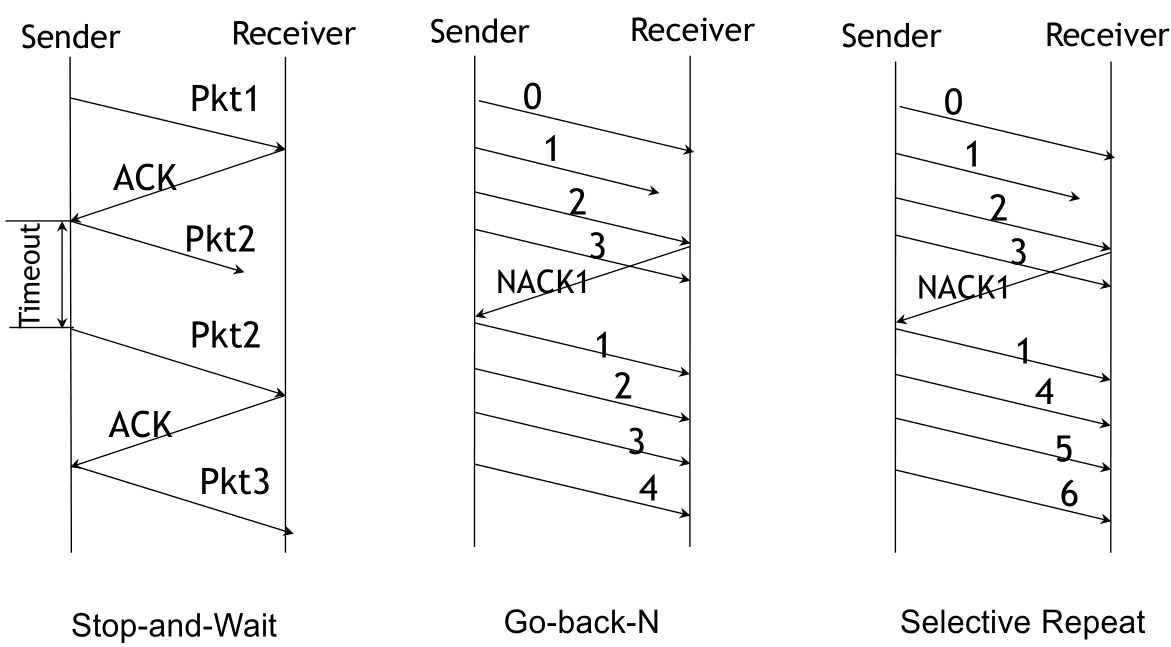
\includegraphics[width=0.7\linewidth]{ARQ}
\caption{Three types of ARQ}
\label{fig:ARQ}
\end{figure}

The last two methods uses negative acknowledgments, which decreases the need for the receiver to transmit packets and thus saves power. The disadvantage is that the sender must keep the last packets send in a buffer, in case a negative acknowledgment is received.

This project focuses on energy comparison between sending compressed and uncompressed data, and not energy savings as such. Therefore the simplest ARQ method is used, namely the Stop-and-Wait. An issue when using this method is to find an optimal timeout period. This is a trade off between reducing idle listening and avoiding collisions of acknowledgments and retransmission. The timeout period in this project is set to 100 ms. This has been empirically tested to be more than sufficient to avoid collisions.

Each packet consists of a fixed size header, a variable size data, possibly a fixed sized footer and metadata. In order to reduce the packet overhead, the data size in each packet was increased to the maximum possible, which in the Tinyos operating system is 112 bytes. This increase the packet error rate.